\chapter{Precipitation and Solubility}\label{ch:b1:precipitation}

A drop of silver nitrate falls into tap water and a white cloud appears:
silver chloride, formed from the few milligrams of chloride ions in every
litre. Water seeping through limestone carries calcium carbonate away and
lays it down again, a fraction of a millimetre a year, as the
stalactites of a cave. A kidney stone is a precipitate too. Each of these
is an equilibrium between a solid and its ions in solution, and one
constant, the \omterm{def:b1:precipitation:solubility-product}{solubility product}, says whether the solid forms, how much
of it dissolves, and how its \omterm{def:b1:precipitation:solubility}{solubility} changes when another ion or the
pH is changed. With it a chemist can separate ions one from another by
precipitating them in turn --- the basis of the treatment of mine
waters that closes this chapter.

\begin{recall}
The school volume (grades 6 and 12) measured \omterm{def:b1:precipitation:solubility}{solubility} in grams per
litre and identified ions by the precipitates they give. The equilibrium
constant, the \omterm{def:b1:extent-q-and-k:quotient}{reaction quotient} $Q$ and the activities (1 for a pure solid
or the solvent, $c/c^\circ$ for a solute) were set up in
\cref{ch:b1:extent-q-and-k}: a reaction goes forward while $Q < K$. The
predominant-reaction method and the scale of $\mathrm{p}K_a$ come from
\cref{ch:b1:predominant-reaction}; $c^\circ = \qty{1}{mol/L}$ is not
written in quotients.
\end{recall}

\begin{omfigure}
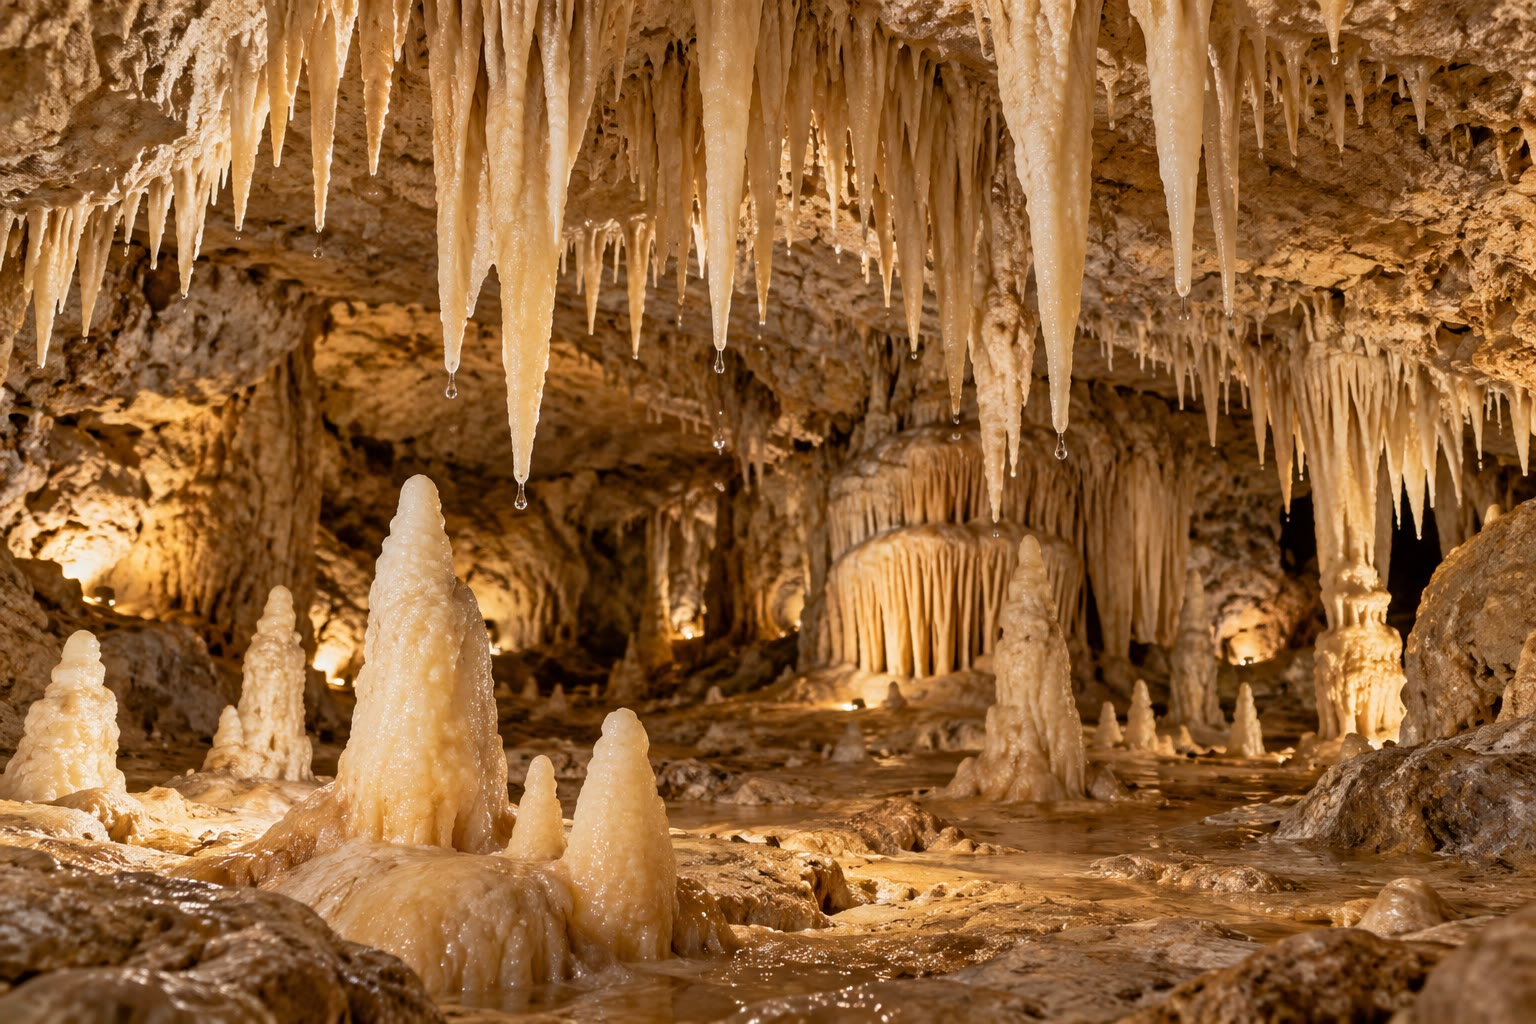
\includegraphics[width=0.62\linewidth]{images/book2/ai/b1-11-cave.jpg}

{\small Stalactites and stalagmites in a limestone cave. Water rich in
carbon dioxide dissolves calcium carbonate in the soil above; in the cave
it loses part of its carbon dioxide and the carbonate precipitates again
(\cref{exo:b1:precipitation:10}).}
\end{omfigure}

\section{The solubility product}\label{sec:b1:precipitation:product}

A \omterm{def:b1:crystals-metals:crystal}{crystal} of silver chloride dropped into water loses ions to the
solution and the solution gives some back to the \omterm{def:b1:crystals-metals:crystal}{crystal}. When the two
rates are equal the solution is \emph{saturated}: its composition no longer
changes, although ions keep passing in both directions
(figure below).

\begin{definition}[Solubility product]\label{def:b1:precipitation:solubility-product}
The \emph{solubility product}\index{solubility product} $K_s$ of an ionic
solid $\mathrm{M}_a\mathrm{X}_b$ is the equilibrium constant of its
dissolution into its ions,
\[
  \mathrm{M}_a\mathrm{X}_b\mathrm{(s)} \rightleftharpoons a\,\mathrm{M}^{m+}
  + b\,\mathrm{X}^{x-}, \qquad
  K_s = [\mathrm{M}^{m+}]_{\mathrm{eq}}^{\,a}\,[\mathrm{X}^{x-}]_{\mathrm{eq}}^{\,b},
  \qquad \mathrm{p}K_s = -\log K_s ,
\]
the \omterm{def:b1:extent-q-and-k:activity}{activity} of the solid being 1. Like every equilibrium constant it
depends on temperature only.
\end{definition}

For silver chloride, \ce{AgCl(s) <=> Ag+ + Cl-} and $K_s =
[\ce{Ag+}][\ce{Cl-}] = 10^{-9.75}$; for calcium fluoride, \ce{CaF2(s) <=>
Ca^2+ + 2F-} and $K_s = [\ce{Ca^2+}][\ce{F-}]^2 = 10^{-9.84}$; for
iron(III) hydroxide, $K_s = [\ce{Fe^3+}][\ce{OH-}]^3 = 10^{-38.55}$.
The table below lists the values used in this volume.
They are computed, like the $\mathrm{p}K_a$ of
\cref{ch:b1:predominant-reaction}, from tabulated standard Gibbs energies
of formation: $\mathrm{p}K_s = \Delta_r G^\circ/(RT\ln 10)$, a relation
derived in the Year~2 volume.

\begin{omfigure}
\begin{tikzpicture}[font=\small, >={Stealth}]
  % the crystal: alternating Ag+ (small, grey) and Cl- (large, green)
  \foreach \i in {0,1,2,3,4,5}
    \foreach \j in {0,1,2} {
      \pgfmathtruncatemacro{\pp}{mod(\i+\j,2)}
      \ifnum\pp=0
        \shade[ball color=green!55!black!60] (\i*0.62,\j*0.62) circle (0.29);
      \else
        \shade[ball color=gray!35] (\i*0.62,\j*0.62) circle (0.17);
      \fi }
  \draw[thick, gray] (-0.45,-0.45) rectangle (3.55,1.75);
  \node[below] at (1.55,-0.45) {\ce{AgCl(s)}};
  % ions in solution
  \shade[ball color=gray!35] (1.2,3.0) circle (0.17);
  \node[right] at (1.4,3.0) {\ce{Ag+}};
  \shade[ball color=green!55!black!60] (2.6,2.7) circle (0.29);
  \node[right] at (2.9,2.7) {\ce{Cl-}};
  \shade[ball color=gray!35] (4.4,1.4) circle (0.17);
  \shade[ball color=green!55!black!60] (5.1,2.6) circle (0.29);
  \shade[ball color=gray!35] (-1.0,2.4) circle (0.17);
  \shade[ball color=green!55!black!60] (-0.6,3.3) circle (0.29);
  % arrows: dissolution and precipitation
  \draw[->, thick, omDef] (1.24,1.6) to[bend left=20] node[left, pos=0.6] {dissolution} (1.15,2.78);
  \draw[->, thick, omProp] (2.55,2.38) to[bend left=20] node[right, pos=0.45] {precipitation} (2.45,1.55);
  % the water line
  \draw[blue!50, thick] (-1.6,3.8) -- (5.9,3.8);
  \node[blue!60!black, anchor=east] at (5.9,4.05) {saturated solution};
\end{tikzpicture}

{\small A \omterm{def:b1:crystals-metals:crystal}{crystal} of silver chloride in its saturated solution. Ions leave
the surface (dissolution) and others are captured (precipitation) at the
same rate, so that $[\ce{Ag+}][\ce{Cl-}]$ stays equal to $K_s$. Silver ions
are drawn smaller than chloride ions, as they are.}
\end{omfigure}

\begin{omfigure}
\begin{tabular}{lc@{\qquad}lc}
\hline
solid & $\mathrm{p}K_s$ & solid & $\mathrm{p}K_s$ \\
\hline
\ce{AgCl} & 9.75 & \ce{Ca(OH)2} & 5.33 \\
\ce{AgBr} & 12.27 & \ce{Mg(OH)2} & 11.25 \\
\ce{AgI} & 16.07 & \ce{Fe(OH)2} & 16.31 \\
\ce{Ag2CrO4} & 11.95 & \ce{Zn(OH)2} & 16.38 \\
\ce{BaSO4} & 9.97 & \ce{Fe(OH)3} & 38.55 \\
\ce{CaCO3} (calcite) & 8.30 & \ce{Al(OH)3} (gibbsite) & 34.75 \\
\ce{CaF2} & 9.84 & & \\
\hline
\end{tabular}

\smallskip
{\small \omterm{def:b1:precipitation:solubility-product}{Solubility products} at \qty{25}{\celsius}, computed from the
standard Gibbs energies of formation of the solids and of the aqueous
ions. Formation constants used in this chapter (\cref{sec:b1:precipitation:amphoteric}):
$\log\beta_4 = 14.45$ for \ce{Zn(OH)4^2-}, 33.52 for \ce{Al(OH)4-}, and
$\log\beta_1 = 11.82$ for \ce{FeOH^2+}.}
% ledger: dfg:AgCl_cr, dfg:AgBr_cr, dfg:AgI_cr, dfg:Ag2CrO4_cr, dfg:Ag+_ao, dfg:Cl-_ao, dfg:Br-_ao, dfg:I-_ao, dfg:CrO42-_ao (computed in figdata/bachelor-1/aqueous-constants.py)
% ledger: dfg:BaSO4_cr, dfg:Ba2+_ao, dfg:SO42-_ao, dfg:CaCO3_cr, dfg:CO32-_ao, dfg:CaF2_cr, dfg:Ca2+_ao, dfg:F-_ao (computed, same script)
% ledger: dfg:Ca_OH2_cr, dfg:Mg_OH2_cr, dfg:Mg2+_ao, dfg:Fe_OH2_cr, dfg:Fe2+_ao, dfg:Zn_OH2_cr, dfg:Zn2+_ao, dfg:Fe_OH3_cr, dfg:Fe3+_ao, dfg:Al2O3.3H2O_cr, dfg:Al3+_ao, dfg:OH-_ao (computed, same script)
% ledger: dfg:Zn_OH42-_ao, dfg:Al_OH4-_ao, dfg:FeOH2+_ao (formation constants, same script)
\end{omfigure}

\begin{proposition}[Condition of precipitation]\label{prop:b1:precipitation:precipitation-condition}
Let a solution contain the ions of a solid $\mathrm{M}_a\mathrm{X}_b$, with
\omterm{def:b1:extent-q-and-k:quotient}{reaction quotient} $Q_s = [\mathrm{M}^{m+}]^a[\mathrm{X}^{x-}]^b$ for the
dissolution.
\begin{itemize}
  \item If $Q_s < K_s$, the solid cannot be present at equilibrium: the
        solution is unsaturated and any solid added dissolves, completely
        if there is not too much of it.
  \item If $Q_s > K_s$, the solid precipitates until $Q_s = K_s$.
  \item The solid and the solution coexist at equilibrium only when
        $Q_s = K_s$.
\end{itemize}
\end{proposition}

\begin{proof}
By \cref{ch:b1:extent-q-and-k}, the dissolution goes forward as long as
$Q_s < K_s$ and backward (precipitation) as long as $Q_s > K_s$. While the
dissolution goes forward, $Q_s$ increases. If the solid is used up before
$Q_s$ reaches $K_s$, the evolution stops with no solid left: a reaction
with a pure condensed \omterm{def:b1:extent-q-and-k:system}{phase} can stop before equilibrium because the
amount of that \omterm{def:b1:extent-q-and-k:system}{phase} cannot become negative. If $Q_s > K_s$, precipitation
lowers both ion concentrations and $Q_s$ decreases until it equals $K_s$,
which it always can, since the ions are there.
\end{proof}

The last point is what distinguishes a solid from a dissolved species. An
acid--base species is present at every pH, however little; a solid is
either present or absent. This is why its diagram will be an
\emph{existence} diagram, not a predominance one
(\cref{sec:b1:precipitation:domains}).

\begin{example}[Mixing two solutions]\label{ex:b1:precipitation:mixing}
\qty{10.0}{mL} of silver nitrate at \qty{2.0e-4}{mol/L} are mixed with
\qty{10.0}{mL} of sodium chloride at \qty{2.0e-4}{mol/L}. Just after
mixing, before any reaction, $[\ce{Ag+}] = [\ce{Cl-}] = \qty{1.0e-4}{mol/L}$
and $Q_s = 10^{-8.0} > K_s = 10^{-9.75}$: silver chloride precipitates.
With both solutions at \qty{2.0e-6}{mol/L}, $Q_s = 10^{-12.0} < K_s$ and the
mixture stays clear. Silver nitrate is a sensitive test for chloride
ions, but not an infinitely sensitive one.
\end{example}

\begin{inthelab}[The chloride test]
In the teaching laboratory, a few drops of silver nitrate solution are
added to the sample, first acidified with dilute nitric acid. The acid
turns carbonate and hydroxide ions into carbon dioxide and water, which
would otherwise also precipitate with silver ions. A white precipitate
that darkens in light is silver chloride; bromide gives a cream
precipitate and iodide a yellow one
(photograph below).
Silver nitrate stains the skin black: gloves and goggles are worn.
\end{inthelab}

\begin{omfigure}
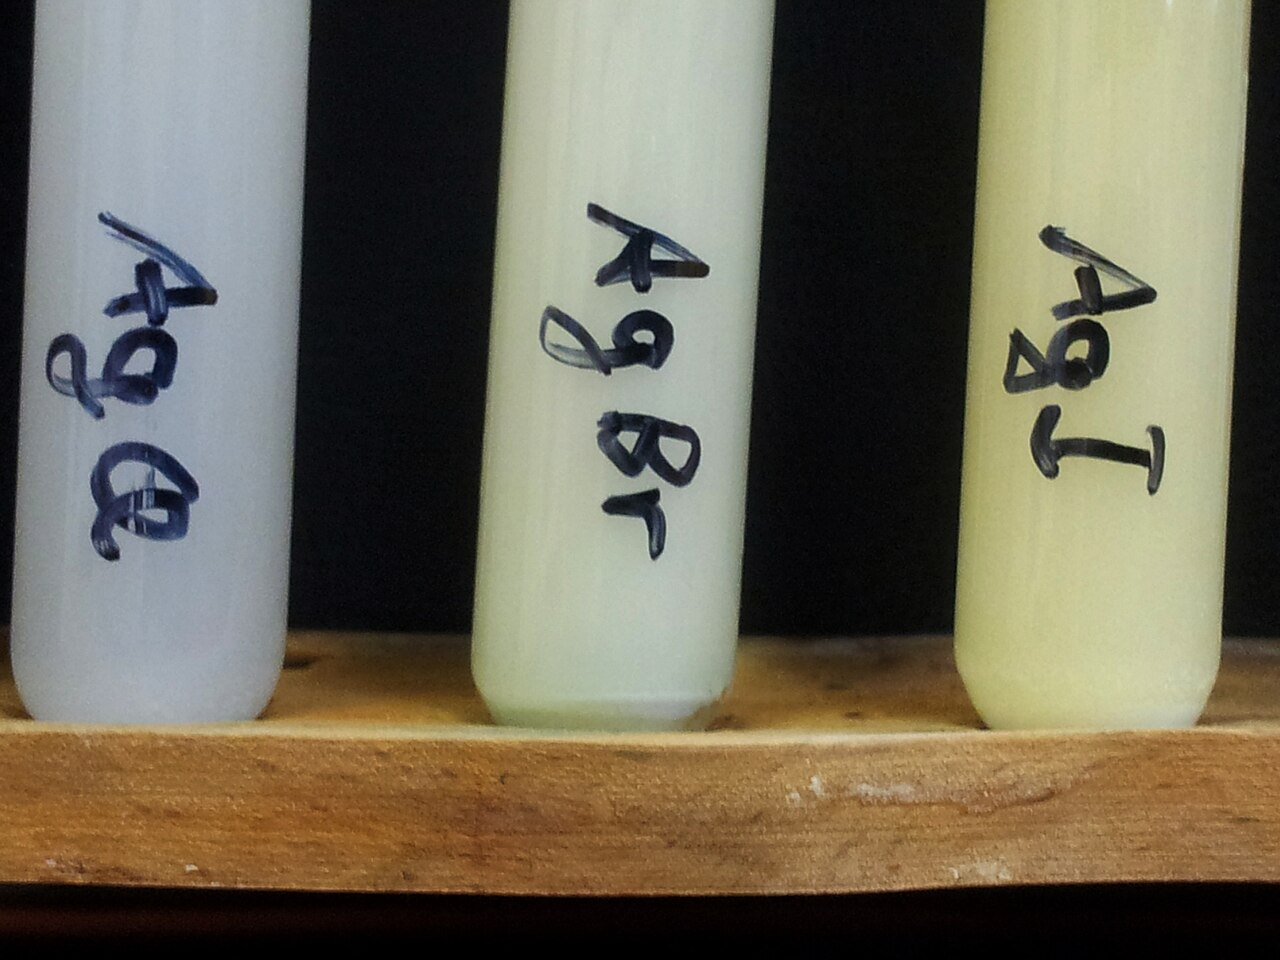
\includegraphics[width=0.6\linewidth]{images/book2/silver-halides.jpg}

{\small Precipitates of silver chloride (white), silver bromide (cream)
and silver iodide (pale yellow). Photograph Rrausch1974, CC BY-SA 3.0,
Wikimedia Commons.}
\end{omfigure}

\section{Solubility}

\begin{definition}[Solubility]\label{def:b1:precipitation:solubility}
The \emph{solubility}\index{solubility} $s$ of a solid in a given solution
is the amount of solid that dissolves in one litre of that solution
until saturation (in \unit{mol/L}); multiplied by the molar mass, it is
the mass solubility, in \unit{g/L}. It depends on the temperature and on
the composition of the solution.
\end{definition}

\begin{proposition}[Solubility from the solubility product]\label{prop:b1:precipitation:s-of-ks}
In pure water, if the ions take part in no other reaction,
\[
  \mathrm{MX}:\ s = \sqrt{K_s}, \qquad
  \mathrm{MX_2}\ \text{or}\ \mathrm{M_2X}:\ s = \left(\frac{K_s}{4}\right)^{1/3},
  \qquad
  \mathrm{M}_a\mathrm{X}_b:\ s = \left(\frac{K_s}{a^a b^b}\right)^{1/(a+b)} .
\]
\end{proposition}

\begin{proof}
When $s$ mol of solid dissolve per litre, $[\mathrm{M}^{m+}] = as$ and
$[\mathrm{X}^{x-}] = bs$, so at saturation $K_s = (as)^a(bs)^b =
a^a b^b s^{a+b}$. For MX, $a = b = 1$; for \ce{MX2}, $1^1 2^2 = 4$, and the
same for \ce{M2X}.
\end{proof}

\begin{example}[Silver chloride and silver chromate]\label{ex:b1:precipitation:agcl-ag2cro4}
Silver chloride: $s = 10^{-9.75/2} = \qty{1.3e-5}{mol/L}$, or
\qty{1.9}{mg/L} with $M = \qty{143.4}{g/mol}$. Silver chromate \ce{Ag2CrO4}
($\mathrm{p}K_s = 11.95$): $s = (10^{-11.95}/4)^{1/3} =
\qty{6.6e-5}{mol/L}$. The chromate has the smaller $K_s$ and yet is five
times more soluble. \omterm{def:b1:precipitation:solubility-product}{Solubility products} can be compared directly only
between solids of the same formula type.
\end{example}

\begin{remark}
The formulas assume that the ions are free. In pure water the chromate
ion is a \omterm{def:b1:predominant-reaction:strong-acid}{weak base} and the silver ion is complexed by nothing, so the
result for silver chromate is close to correct; for a carbonate, a
sulfide or a hydroxide the base properties of the anion matter and the
next section is needed. At high ionic strength the activities also drift
away from the concentrations, a correction left to the Year~2 volume.
\end{remark}

\section{Common-ion and pH effects}

\begin{definition}[Common-ion effect]\label{def:b1:precipitation:common-ion}
The \emph{common-ion effect}\index{common-ion effect} is the decrease of
the \omterm{def:b1:precipitation:solubility}{solubility} of a solid in a solution that already contains one of its
ions.
\end{definition}

\begin{proposition}[Solubility with a common ion]\label{prop:b1:precipitation:common-ion}
Let MX dissolve in a solution where $[\mathrm{X}^-] = c$ already, with
$c \gg \sqrt{K_s}$. Then $s \approx K_s/c$, much smaller than in pure
water. For \ce{MX2} in a solution containing \ce{M^2+} at $c$,
$s \approx \frac12\sqrt{K_s/c}$.
\end{proposition}

\begin{proof}
At saturation $[\mathrm{M}^+] = s$ and $[\mathrm{X}^-] = c + s$, so
$s(c + s) = K_s$. If $s \ll c$, $s = K_s/c$; the assumption holds since
$K_s/c \ll c$ when $c^2 \gg K_s$. For \ce{MX2}, $[\ce{X-}] = 2s$ and
$[\mathrm{M}^{2+}] = c + s \approx c$, so $c\,(2s)^2 = K_s$.
\end{proof}

Silver chloride in \qty{0.10}{mol/L} sodium chloride: $s = 10^{-9.75}/0.10
= \qty{1.8e-9}{mol/L}$, seven thousand times less than in water. This is
why a precipitate is washed with a dilute solution of a common ion rather
than with pure water: it loses less of itself.

When the anion of the solid is a base, acid pulls it out of the
dissolution equilibrium and the \omterm{def:b1:precipitation:solubility}{solubility} rises. For calcium carbonate in
acid,
\[
  \ce{CaCO3(s) + H3O+ <=> Ca^2+ + HCO3- + H2O}, \qquad
  K = \frac{K_s}{K_{a2}} = 10^{-8.30 + 10.33} = 10^{2.03} ,
\]
a favoured reaction: vinegar or hydrochloric acid dissolves limestone,
and the carbon dioxide formed by the further reaction of
\ce{HCO3-} gives the familiar fizz.
% ledger: dfg:HCO3-_ao (pKa2 of carbonic acid, ch. 10)

\begin{proposition}[Solubility of a hydroxide against pH]\label{prop:b1:precipitation:hydroxide-ph}
In a solution buffered at a given pH, the concentration of \ce{M^{n+}} in
equilibrium with the hydroxide \ce{M(OH)_n} obeys
\[
  \log[\mathrm{M}^{n+}] = -\mathrm{p}K_s + n\,(\mathrm{p}K_e - \mathrm{pH}) ,
\]
a straight line of slope $-n$ against pH. If the ion forms no complex,
this is the \omterm{def:b1:precipitation:solubility}{solubility} of the hydroxide.
\end{proposition}

\begin{proof}
$K_s = [\mathrm{M}^{n+}][\ce{OH-}]^n$ and $[\ce{OH-}] = K_e/[\ce{H3O+}]$,
so $\log[\mathrm{M}^{n+}] = \log K_s - n\log[\ce{OH-}] = -\mathrm{p}K_s -
n(\mathrm{pH} - \mathrm{p}K_e)$.
\end{proof}

Each unit of pH divides the \omterm{def:b1:precipitation:solubility}{solubility} of iron(III) hydroxide by a
thousand and that of zinc hydroxide by a hundred. Hydroxides are
precipitated, and dissolved again, by changing the pH.

\begin{example}[Dissolving calcium carbonate with carbon dioxide]\label{ex:b1:precipitation:cave}
Water containing dissolved carbon dioxide dissolves calcite:
\[
  \ce{CaCO3(s) + CO2(aq) + H2O <=> Ca^2+ + 2HCO3-}, \qquad
  K = \frac{K_s K_{a1}}{K_{a2}} = 10^{-8.30 - 6.37 + 10.33} = 10^{-4.34} ,
\]
the constant being obtained by adding the dissolution of the carbonate,
the first acidity of carbon dioxide and the reverse of the second. The
more carbon dioxide, the more calcium carbonate dissolves. Soil air is usually
far richer in carbon dioxide than the air of a cave; water that has
crossed the soil and reaches the cave ceiling loses carbon dioxide, and
calcite deposits (\cref{exo:b1:precipitation:10}).
\end{example}

\section{Existence domains and selective precipitation}\label{sec:b1:precipitation:domains}

\begin{definition}[Existence domain]\label{def:b1:precipitation:existence-domain}
For a solid and a given total concentration $c$ of one of its ions, the
\emph{existence domain}\index{existence domain} of the solid is the range
of the variable (pX, pM or pH) over which the solid is present at
equilibrium. Its boundary is the value at which the first grain of solid
appears, when $Q_s = K_s$ with the ion still at concentration $c$.
\end{definition}

\begin{method}[Drawing an existence diagram]\label{met:b1:precipitation:existence-domain}
\begin{enumerate}
  \item Fix the total concentration $c$ of the ion that is not on the
        axis (for instance $[\ce{Ag+}]_{\mathrm{tot}} = c$ on a pCl axis).
  \item Write $K_s$ at the onset of precipitation, with that ion still at
        $c$, and solve for the variable on the axis.
  \item The solid exists on the side where the other ion is
        concentrated: small pCl (much chloride), small pAg, or high pH
        for a hydroxide.
  \item Do not mark a domain for the ion itself: it is present
        everywhere, at $c$ outside the domain of the solid and below $c$
        inside it.
\end{enumerate}
\end{method}

For silver chloride with $c = [\ce{Ag+}]_{\mathrm{tot}} = 10^{-2}$:
precipitation starts when $[\ce{Cl-}] = K_s/c = 10^{-7.75}$, so the solid
exists for $\mathrm{pCl} < 7.75$. For silver iodide the boundary is at
$\mathrm{pI} = 16.07 - 2 = 14.07$, as drawn below.

\begin{omfigure}
\begin{tikzpicture}[font=\small, >={Stealth}, x=0.62cm]
  \fill[omDef!18] (0,0.12) rectangle (7.75,0.6);
  \draw[->, thick] (0,0) -- (17.2,0) node[right] {pCl or pI};
  \foreach \x in {0,2,4,6,8,10,12,14,16}
    \draw (\x,0.08) -- (\x,-0.08) node[below] {\x};
  \draw[omDef, thick] (7.75,-0.5) -- (7.75,0.9);
  \node[omDef] at (3.9,0.36) {\ce{AgCl(s)} exists};
  \node[omDef, above] at (7.75,0.9) {7.75};
  \node[anchor=west] at (8.0,0.36) {no solid: \ce{Ag+} at $10^{-2}$ mol/L};
  % AgI below
  \begin{scope}[yshift=-1.9cm]
  \fill[omProp!20] (0,0.12) rectangle (14.07,0.6);
  \draw[->, thick] (0,0) -- (17.2,0);
  \foreach \x in {0,2,4,6,8,10,12,14,16}
    \draw (\x,0.08) -- (\x,-0.08) node[below] {\x};
  \draw[omProp, thick] (14.07,-0.5) -- (14.07,0.9);
  \node[omProp] at (7.0,0.36) {\ce{AgI(s)} exists};
  \node[omProp, above] at (14.07,0.9) {14.07};
  \end{scope}
\end{tikzpicture}

{\small \omterm{def:b1:precipitation:existence-domain}{Existence domains} of silver chloride (on a pCl axis, top) and
silver iodide (on a pI axis, bottom) for a total silver concentration
of \qty{1.0e-2}{mol/L}. Iodide precipitates silver at concentrations a
million times lower than chloride does.}
\end{omfigure}

\begin{method}[Selective precipitation]\label{met:b1:precipitation:selective}
To separate two ions that precipitate with the same reagent:
\begin{enumerate}
  \item compute, for each ion at its concentration, the reagent
        concentration (or pH) at which its solid starts to form; the
        lower one precipitates first;
  \item compute the concentration of the first ion left in solution when
        the second starts to precipitate;
  \item the separation is acceptable if that concentration is a small
        enough fraction of the initial one --- typically \qty{0.1}{\percent}
        --- and the reagent is then stopped between the two thresholds.
\end{enumerate}
\end{method}

\begin{example}[Iodide and chloride]\label{ex:b1:precipitation:i-cl}
A solution contains iodide and chloride ions, both at
\qty{1.0e-2}{mol/L}; silver nitrate is added drop by drop, without
dilution. Silver iodide starts to form at $[\ce{Ag+}] = 10^{-16.07 + 2} =
10^{-14.07}$, silver chloride at $10^{-9.75 + 2} = 10^{-7.75}$: iodide
precipitates first. When silver chloride appears,
$[\ce{I-}] = 10^{-16.07}/10^{-7.75} = 10^{-8.32} = \qty{4.8e-9}{mol/L}$,
a fraction $5 \times 10^{-7}$ of the iodide: the separation is complete.
\end{example}

Hydroxides are separated in the same way with the pH as the variable.
The chart below shows, for six ions at
\qty{0.010}{mol/L}, the pH where the hydroxide appears and the pH where
\qty{99.9}{\percent} of the ion has precipitated. Iron(III) and aluminium are
removed in acidic water, zinc and iron(II) near neutrality, magnesium
around pH 10 and calcium only in very basic water.

\begin{omfigure}
\begin{tikzpicture}
\begin{axis}[
  width=0.82\linewidth, height=5.4cm, xmin=0, xmax=14, ymin=0.4, ymax=6.6,
  axis x line=bottom, axis y line=left, xlabel={pH},
  xtick={0,2,4,6,8,10,12,14}, ytick={1,2,3,4,5,6},
  yticklabels={\ce{Fe^3+}, \ce{Al^3+}, \ce{Zn^2+}, \ce{Fe^2+}, \ce{Mg^2+}, \ce{Ca^2+}},
  y dir=reverse, axis line style={-},
  tick label style={font=\small}, label style={font=\small}]
\addplot[draw=none, omDef!35,
  error bars/.cd, x dir=plus, x explicit,
  error bar style={line width=7pt, omDef!35}, error mark=none]
  table[x=start, y=row, x error expr=14-\thisrow{start}] {figdata/out/bachelor-1-solubility-ph-thresholds.dat};
\addplot[draw=none, omDef,
  error bars/.cd, x dir=plus, x explicit,
  error bar style={line width=7pt, omDef}, error mark=none]
  table[x=start, y=row, x error expr=\thisrow{end}-\thisrow{start}] {figdata/out/bachelor-1-solubility-ph-thresholds.dat};
\end{axis}
\end{tikzpicture}

{\small Precipitation of hydroxides from solutions at \qty{0.010}{mol/L} of
each ion. The dark bar runs from the first grain of hydroxide to the pH
where \qty{99.9}{\percent} of the ion is precipitated (one pH unit wide for a
trivalent ion, one and a half for a divalent one); the light bar is the
rest of the \omterm{def:b1:precipitation:existence-domain}{existence domain} of the hydroxide. The amphoteric
redissolution of zinc and aluminium hydroxides at high pH
(\cref{sec:b1:precipitation:amphoteric}) is not shown.}
\end{omfigure}

\section{Amphoteric hydroxides}\label{sec:b1:precipitation:amphoteric}

Add sodium hydroxide drop by drop to a solution of zinc sulfate: a white
precipitate of zinc hydroxide forms, then, in excess hydroxide, it
dissolves again. Aluminium hydroxide does the same; iron(III) and
magnesium hydroxides do not.

\begin{definition}[Amphoteric hydroxide]\label{def:b1:precipitation:amphoteric-hydroxide}
A hydroxide is an \emph{amphoteric hydroxide}\index{amphoteric hydroxide}
if it dissolves both in acid, as the cation, and in excess base, as a
hydroxo complex anion:
\[
  \ce{Zn(OH)2(s) + 2H3O+ -> Zn^2+ + 4H2O}, \qquad
  \ce{Zn(OH)2(s) + 2OH- -> Zn(OH)4^2-} .
\]
\end{definition}

The complex anion \ce{Zn(OH)4^2-} (tetrahydroxozincate) is characterised by
its formation constant $\beta_4 = [\ce{Zn(OH)4^2-}]/([\ce{Zn^2+}][\ce{OH-}]^4)
= 10^{14.45}$; complexes and their constants are the subject of
\cref{ch:b1:complexation}.

\begin{proposition}[Solubility of an amphoteric hydroxide]\label{prop:b1:precipitation:amphoteric}
If zinc is in solution only as \ce{Zn^2+} and \ce{Zn(OH)4^2-}, the
\omterm{def:b1:precipitation:solubility}{solubility} of zinc hydroxide is
\[
  s = [\ce{Zn^2+}] + [\ce{Zn(OH)4^2-}] = \frac{K_s}{[\ce{OH-}]^2} + K\,[\ce{OH-}]^2,
  \qquad K = \beta_4 K_s = 10^{-1.93} .
\]
In $\log s$ against pH it follows a line of slope $-2$ at low pH and a line
of slope $+2$ at high pH. It is smallest at
$[\ce{OH-}]^4 = K_s/K = 1/\beta_4$, that is at $\mathrm{pH} =
\mathrm{p}K_e - \frac14\log\beta_4$, where $s_{\min} = 2\sqrt{K_s K}$.
\end{proposition}

\begin{proof}
At saturation $[\ce{Zn^2+}] = K_s/[\ce{OH-}]^2$, and
$[\ce{Zn(OH)4^2-}] = \beta_4[\ce{Zn^2+}][\ce{OH-}]^4 = \beta_4 K_s
[\ce{OH-}]^2$. With $w = [\ce{OH-}]^2$, $s(w) = K_s/w + Kw$ has derivative
$-K_s/w^2 + K$, zero at $w = \sqrt{K_s/K}$, where $s = 2\sqrt{K_s K}$. At
low pH the first term dominates and $\log s = \log K_s - 2\log[\ce{OH-}]$
(slope $-2$ in pH); at high pH the second, $\log s = \log K + 2\log[\ce{OH-}]$
(slope $+2$).
\end{proof}

With the values above, the minimum lies at $\mathrm{pH} = 14.00 - 14.45/4
= 10.39$ and $s_{\min} = 2 \times 10^{-(16.38 + 1.93)/2} =
\qty{1.4e-9}{mol/L}$
(figure below). The real
minimum is far higher: zinc also forms \ce{ZnOH+}, \ce{Zn(OH)3-} and,
above all, an uncharged dissolved \ce{Zn(OH)2(aq)}, whose concentration in
equilibrium with the solid does not depend on the pH. The full
calculation, with the same tables, puts the floor near
$10^{-5.6}$~mol/L. A two-species model gives the slopes and the order of
the thresholds; near the minimum every species counts.

\begin{omfigure}
\begin{tikzpicture}
\begin{axis}[name=zn,
  width=0.46\linewidth, height=5.6cm, xmin=6, xmax=14, ymin=-10, ymax=0,
  axis x line=bottom, axis y line=left, xlabel={pH}, ylabel={$\log s$},
  xtick={6,8,10,12,14}, ytick={-10,-8,-6,-4,-2,0},
  tick label style={font=\small}, label style={font=\small}]
\addplot[omProp, dashed, thick] table[x=pH, y=full] {figdata/out/bachelor-1-solubility-ph-zinc.dat};
\addplot[omDef, very thick] table[x=pH, y=model] {figdata/out/bachelor-1-solubility-ph-zinc.dat};
\node[font=\small, anchor=west] at (axis cs:7.0,-1.0) {\ce{Zn^2+}};
\node[font=\small, anchor=east] at (axis cs:13.8,-1.1) {\ce{Zn(OH)4^2-}};
\node[font=\small, omProp, anchor=south] at (axis cs:10.4,-5.5) {all species};
\node[font=\small, anchor=north] at (axis cs:10.2,-0.4) {zinc};
\end{axis}
\begin{axis}[at={(zn.east)}, anchor=west, xshift=1.8cm,
  width=0.46\linewidth, height=5.6cm, xmin=2, xmax=14, ymin=-10, ymax=0,
  axis x line=bottom, axis y line=left, xlabel={pH}, ylabel={$\log s$},
  xtick={2,4,6,8,10,12,14}, ytick={-10,-8,-6,-4,-2,0},
  tick label style={font=\small}, label style={font=\small}]
\addplot[omDef, very thick] table[x=pH, y=model] {figdata/out/bachelor-1-solubility-ph-aluminium.dat};
\node[font=\small, anchor=west] at (axis cs:3.4,-0.8) {\ce{Al^3+}};
\node[font=\small, anchor=east] at (axis cs:13.8,-0.6) {\ce{Al(OH)4-}};
\node[font=\small, anchor=north] at (axis cs:8.6,-0.4) {aluminium};
\end{axis}
\end{tikzpicture}

{\small \omterm{def:b1:precipitation:solubility}{Solubility} of zinc hydroxide (left) and of aluminium hydroxide,
gibbsite (right), against pH, two-species model (solid lines): slopes
$-2$ and $+2$ for zinc, $-3$ and $+1$ for aluminium. For zinc the dashed curve includes all the
hydroxo species, the uncharged \ce{Zn(OH)2(aq)} setting a floor.}
\end{omfigure}

For aluminium the hydroxide is \ce{Al(OH)3} and the complex \ce{Al(OH)4-},
so $\ce{Al(OH)3(s) + OH- <=> Al(OH)4-}$ with $K = \beta_4 K_s = 10^{33.52
- 34.75} = 10^{-1.23}$ and slopes $-3$ and $+1$. The difference between
aluminium and iron(III) --- one amphoteric, the other not --- is used
industrially to separate them: hot sodium hydroxide dissolves the
aluminium of bauxite and leaves the iron oxides behind
(\cref{exo:b1:precipitation:12}).

\section{Exercises}

\begin{exercise}[$\star$]\label{exo:b1:precipitation:1}
Write the dissolution equation and the expression of $K_s$ for
\ce{BaSO4}, \ce{CaF2}, \ce{Ag2CrO4} and \ce{Fe(OH)3}. Give $K_s$ in powers
of ten from the table of \cref{sec:b1:precipitation:product}, and the $\mathrm{p}K_s$ of a
solid of $K_s = \num{2.0e-13}$.
\end{exercise}

\begin{exercise}[$\star$]\label{exo:b1:precipitation:2}
Compute the \omterm{def:b1:precipitation:solubility}{solubility} of silver bromide in pure water in \unit{mol/L}
and in \unit{mg/L} ($M = \qty{187.8}{g/mol}$).
\end{exercise}

\begin{exercise}[$\star$]\label{exo:b1:precipitation:3}
\qty{50}{mL} of barium chloride at \qty{2.0e-3}{mol/L} are mixed with
\qty{50}{mL} of sodium sulfate at \qty{2.0e-4}{mol/L}. Does barium
sulfate precipitate? Same question with sodium sulfate at
\qty{2.0e-7}{mol/L}.
\end{exercise}

\begin{exercise}[$\star$]\label{exo:b1:precipitation:4}
Compute the \omterm{def:b1:precipitation:solubility}{solubility} of barium sulfate in pure water, then in a
solution of sodium sulfate at \qty{0.010}{mol/L}. By what factor has it
changed?
\end{exercise}

\begin{exercise}[$\star\star$]\label{exo:b1:precipitation:5}
Compute the \omterm{def:b1:precipitation:solubility}{solubility} of calcium fluoride in pure water (\unit{mol/L} and
\unit{mg/L}, $M = \qty{78.1}{g/mol}$), then in a solution of calcium
chloride at \qty{0.10}{mol/L}. Check the approximation you made.
\end{exercise}

\begin{exercise}[$\star\star$]\label{exo:b1:precipitation:6}
A solution contains magnesium ions at \qty{0.050}{mol/L}. At what pH does
magnesium hydroxide start to precipitate? At what pH is \qty{99}{\percent} of
the magnesium precipitated? Draw the \omterm{def:b1:precipitation:existence-domain}{existence domain} of \ce{Mg(OH)2} on a
pH axis.
\end{exercise}

\begin{exercise}[$\star\star$]\label{exo:b1:precipitation:7}
A solution contains bromide and chloride ions, both at
\qty{1.0e-2}{mol/L}. Silver nitrate is added without dilution. Which
precipitate appears first? What fraction of the first ion is still in
solution when the second solid appears? Is the separation acceptable?
\end{exercise}

\begin{exercise}[$\star\star$]\label{exo:b1:precipitation:8}
The Mohr titration of chloride by silver ions uses chromate ions as the
indicator: red silver chromate must appear only once nearly all the
chloride has precipitated. Chloride is at \qty{0.050}{mol/L} and chromate
at \qty{5.0e-3}{mol/L}; dilution is neglected. Compute $[\ce{Ag+}]$ when
silver chromate starts to form, and the fraction of chloride still in
solution at that moment.
\end{exercise}

\begin{exercise}[$\star\star$]\label{exo:b1:precipitation:9}
Calcium carbonate is shaken with a solution kept at pH 8.30 by a buffer,
where hydrogencarbonate is by far the main carbonate species. Show that
$[\ce{Ca^2+}][\ce{HCO3-}] = K_s\,10^{\mathrm{p}K_{a2} - \mathrm{pH}}$, and
compute the \omterm{def:b1:precipitation:solubility}{solubility}, assuming that all the carbonate dissolved stays
as \ce{HCO3-} ($\mathrm{p}K_{a2} = 10.33$).
\end{exercise}

\begin{exercise}[$\star\star\star$]\label{exo:b1:precipitation:10}
Limestone caves. The \omterm{def:b1:precipitation:solubility}{solubility} of carbon dioxide follows
\ce{CO2(g) <=> CO2(aq)} with $\log K_H = -1.47$ ($K_H =
[\ce{CO2(aq)}]/p(\ce{CO2})$, pressure in bar).
\begin{enumerate}
  \item Combine $K_H$ with the constant of
        \cref{ex:b1:precipitation:cave} to obtain the constant of
        \ce{CaCO3(s) + CO2(g) + H2O <=> Ca^2+ + 2HCO3-}.
  \item Show that the \omterm{def:b1:precipitation:solubility}{solubility} of calcite is $s = (K'p/4)^{1/3}$ and
        compute it in water that has equilibrated with soil air at
        $p(\ce{CO2}) = \qty{0.010}{bar}$, then with outdoor air,
        \qty{4.26e-4}{bar}. Give both in \unit{mg/L} of \ce{CaCO3}
        ($M = \qty{100.1}{g/mol}$).
  \item Explain the growth of a stalactite.
\end{enumerate}
\end{exercise}

\begin{exercise}[$\star\star\star$]\label{exo:b1:precipitation:11}
A solution of zinc at \qty{1.0e-2}{mol/L} is brought to increasing pH,
zinc being present only as \ce{Zn^2+} and \ce{Zn(OH)4^2-}.
\begin{enumerate}
  \item Between which pH values is zinc hydroxide present?
  \item Find the pH of minimum \omterm{def:b1:precipitation:solubility}{solubility} and the minimum \omterm{def:b1:precipitation:solubility}{solubility}.
  \item Sketch $\log s$ against pH and label the slopes.
\end{enumerate}
\end{exercise}

\begin{exercise}[$\star\star\star$]\label{exo:b1:precipitation:12}
A solution contains aluminium and iron(III) ions, each at
\qty{1.0e-3}{mol/L}. Sodium hydroxide is added in excess.
\begin{enumerate}
  \item Above what pH is all the aluminium dissolved as \ce{Al(OH)4-}?
  \item What is then the concentration of \ce{Fe^3+}? Conclude about the
        separation.
  \item Explain why the separation would fail with magnesium in place of
        aluminium.
\end{enumerate}
\end{exercise}

\section{Problem: Cleaning a Mine Effluent}

\begin{problem}[{Weekend problem --- precipitation thresholds of three
hydroxides, the hydroxo complex of iron(III), the recovery of zinc and
its amphoteric redissolution, and the pH window for removing iron(III)
without losing zinc(II)}]
\label{pb:b1:precipitation:1}
Water draining from an old metal mine is acidic (pH 2.0) and contains
iron(III) at \qty{1.0e-3}{mol/L}, zinc(II) at \qty{5.0e-3}{mol/L} and
magnesium at \qty{2.0e-2}{mol/L}. The plant raises the pH step by step to
remove the iron as a waste sludge, then to recover the zinc as its
hydroxide, leaving the harmless magnesium in the water. Data at
\qty{25}{\celsius}: $\mathrm{p}K_s$ of \ce{Fe(OH)3} 38.55, \ce{Zn(OH)2}
16.38, \ce{Mg(OH)2} 11.25; $\log\beta_4(\ce{Zn(OH)4^2-}) = 14.45$;
$\log\beta_1(\ce{FeOH^2+}) = 11.82$; $\mathrm{p}K_e = 14.00$; molar masses
\ce{Fe(OH)3} \qty{106.8}{g/mol}, \ce{Zn(OH)2} \qty{99.4}{g/mol}.

\medskip
\noindent\textbf{Part I --- Which hydroxide first?}
\begin{enumerate}
  \item Write the dissolution equilibria of the three hydroxides and
        their $K_s$.
  \item Explain why the three $\mathrm{p}K_s$ alone do not say which
        hydroxide precipitates first.
  \item Show that \ce{M(OH)_n} starts to precipitate from a solution of
        \ce{M^{n+}} at $c$ at $\mathrm{pH} = \mathrm{p}K_e -
        \frac1n(\mathrm{p}K_s + \log c)$.
  \item Compute this pH for iron(III).
  \item Compute it for zinc.
  \item Compute it for magnesium.
  \item Give the order of precipitation as the pH rises. Is anything
        precipitated in the effluent as it leaves the mine?
\end{enumerate}

\medskip
\noindent\textbf{Part II --- Removing iron: first estimate.}
\begin{enumerate}[resume]
  \item The plant wants \qty{99.9}{\percent} of the iron out of the water. What
        concentration of dissolved iron does that allow?
  \item Neglecting any complex, at what pH is this reached?
  \item Show that, in the \omterm{def:b1:precipitation:existence-domain}{existence domain} of \ce{Fe(OH)3},
        $\log[\ce{Fe^3+}]$ decreases by 3 per pH unit.
  \item Up to what pH does the zinc stay entirely in solution?
  \item Give the first estimate of the pH window in which iron is removed
        while zinc stays.
\end{enumerate}

\medskip
\noindent\textbf{Part III --- The hydroxo complex of iron(III).}
\begin{enumerate}[resume]
  \item Write the formation of \ce{FeOH^2+} from \ce{Fe^3+} and \ce{OH-},
        and its constant.
  \item Draw the \omterm{def:b1:predominant-reaction:predominance}{predominance diagram} of \ce{Fe^3+} and \ce{FeOH^2+}
        against pH.
  \item At the pH found in question 9, compute
        $[\ce{FeOH^2+}]/[\ce{Fe^3+}]$. Was the first estimate safe?
  \item Express the total dissolved iron $[\ce{Fe^3+}] + [\ce{FeOH^2+}]$
        in equilibrium with \ce{Fe(OH)3} as a function of the pH.
  \item Show that, where \ce{FeOH^2+} predominates, its logarithm
        decreases by 2 per pH unit.
  \item Find the pH at which the total dissolved iron falls to the value
        of question 8.
\end{enumerate}

\medskip
\noindent\textbf{Part IV --- Recovering zinc.}
\begin{enumerate}[resume]
  \item After the iron sludge is filtered off, the pH is raised again. At
        what pH is \qty{99}{\percent} of the zinc precipitated? Does magnesium
        hydroxide form at that pH?
  \item Write the reaction of zinc hydroxide with excess hydroxide ions
        and compute its constant.
  \item Above what pH would all the zinc be back in solution? What does
        this mean for the operator?
  \item Compute the mass of iron(III) hydroxide sludge removed per cubic
        metre of effluent.
  \item Compute the mass of zinc hydroxide recovered per cubic metre at
        the pH of question 19.
  \item Why must the iron be removed before the zinc, and not both
        together?
  \item State the pH window, to two decimals, in which the iron(III) is
        removed to \qty{99.9}{\percent} while the zinc(II) stays entirely in
        solution.
\end{enumerate}
\end{problem}
